\documentclass[a4paper,12pt]{article}
\usepackage[english,vietnamese]{babel}
\usepackage{amsmath}
\usepackage{booktabs}
\usepackage{graphicx}
\usepackage{hyperref}
\usepackage{lmodern}
\usepackage[nottoc,numbib]{tocbibind}
\renewcommand{\thefootnote}{\fnsymbol{footnote}}

\begin{document}
\setcounter{page}{0}
\thispagestyle{empty}
\vspace*{\stretch{1}}
\begin{flushright}
  \setlength{\baselineskip}{1.4\baselineskip}
\textbf{\Huge Color Image Processing}
  \noindent\rule{\textwidth}{5pt}
  \emph{\Large Digital Image Processing}
  \vspace{\stretch{1}}

  \textbf{by Trần Minh Hiếu, Nguyễn Gia Phong, Nguyễn Văn Tùng,\\
          Nguyễn An Thiết and Nguyễn Thành Vinh\\}
  \selectlanguage{english}
  \today
\end{flushright}
\vspace*{\stretch{2}}
\pagebreak

\selectlanguage{english}
\tableofcontents
\pagebreak

\section{Introduction}
\subsection{Brief Description}
Color images existed long before the rise of computing and digital image
processing.  While most techniques of monochrome image processing such as
blur and edge detection can be directly applied to color images, others
require modification.  Furthermore, there exists procedures specific only
to color images.  In this project, we try to implement some of these
techniques and note down our findings.

This report is licensed under a CC BY-SA 4.0 license, while the source code
is available on GitHub\footnote{\url{https://github.com/McSinyx/recipe}}
under AGPLv3+.

\selectlanguage{vietnamese}
\subsection{Authors and Credits}
The work has been undertaken by group number 8, whose members are listed
in the following table.
\begin{center}
  \begin{tabular}{c c}
    \toprule
    Full name & Student ID\\
    \midrule
    Trần Minh Hiếu & BI9-101\\
    Nguyễn Gia Phong & BI9-184\\
    Nguyễn Văn Tùng & BI9-229\\
    Nguyễn An Thiết & BI8-174\\
    Nguyễn Thành Vinh & BI8-187\\
    \bottomrule
  \end{tabular}
\end{center}

We would like to express our special thanks to Dr.~Nghiêm Thị Phương,
whose lectures gave us basic understanding on the key principles of
digital image processing.  The color image processing lecture notes from
the UMSL's CS 5420 course~\cite{cs5420} also help us gain initial intuition
on the matter.

\newpage
\selectlanguage{english}
\section{Color Spaces}

\section{Color Image Enhancements}

\section{Pseudo Color Rendering}
By mapping each intensity level to a color, one may derive a pseudo color image
from a greyscale images.  Typical usage of such technique is in thermal imaging,
elevation and medical imaging to help the human visual system pick out detail,
estimate quantitative values, and notice patterns in data in a more intuitive
fashion~\cite{turbo}.

In OpenCV, this is available under \verb|applyColorMap|.  It is also trival
to reimplement this function only using NumPy:
\begin{verbatim}
import numpy as np

def map_color(grey, mapping):
    r = np.vectorize(lambda i: mapping[i][0])
    g = np.vectorize(lambda i: mapping[i][1])
    b = np.vectorize(lambda i: mapping[i][2])
    # OpenCV uses BGR by default for whatever reason.
    return np.stack((b(grey), g(grey), r(grey)), axis=-1)
\end{verbatim}

For demonstration, we are going to use the Turbo colormap~\cite{turbo}.
We initially considered solely changing the hue based on intensity,
which is also known as the rainbow map, however it is not a visually
intuitive mapping~\cite{rainbowbad}.

Firstly, we tried to apply the mapping on the heightmap of mainland Vietnam and
its neighboring regions\footnote{The original images are taken from
heightmapper: \url{https://tangrams.github.io/heightmapper/}}.  As seen in
the side-by-side comparison, the colormapped image allows the human eyes
to notice more details, especially the high mountains in the north and
the Khorat Plateau (center of the image).
\begin{center}
  \includegraphics[width=0.49\textwidth]{heightmap-grey.png}
  \includegraphics[width=0.49\textwidth]{heightmap-turbo.png}
\end{center}

In addition, we experimented with pseudo lighting, that is, use colormaps
in place of normal greyscale lighting.  The experiment was carried out on
Phong's game Axuy, where colormapping proved to be an enhancement on helping
players detecting shooting range (Axuy is a first person shooter game).
The video where the game is in action is available on
YouTube\footnote{\url{https://www.youtube.com/watch?v=QVGAaoordpk}}.
\begin{center}
  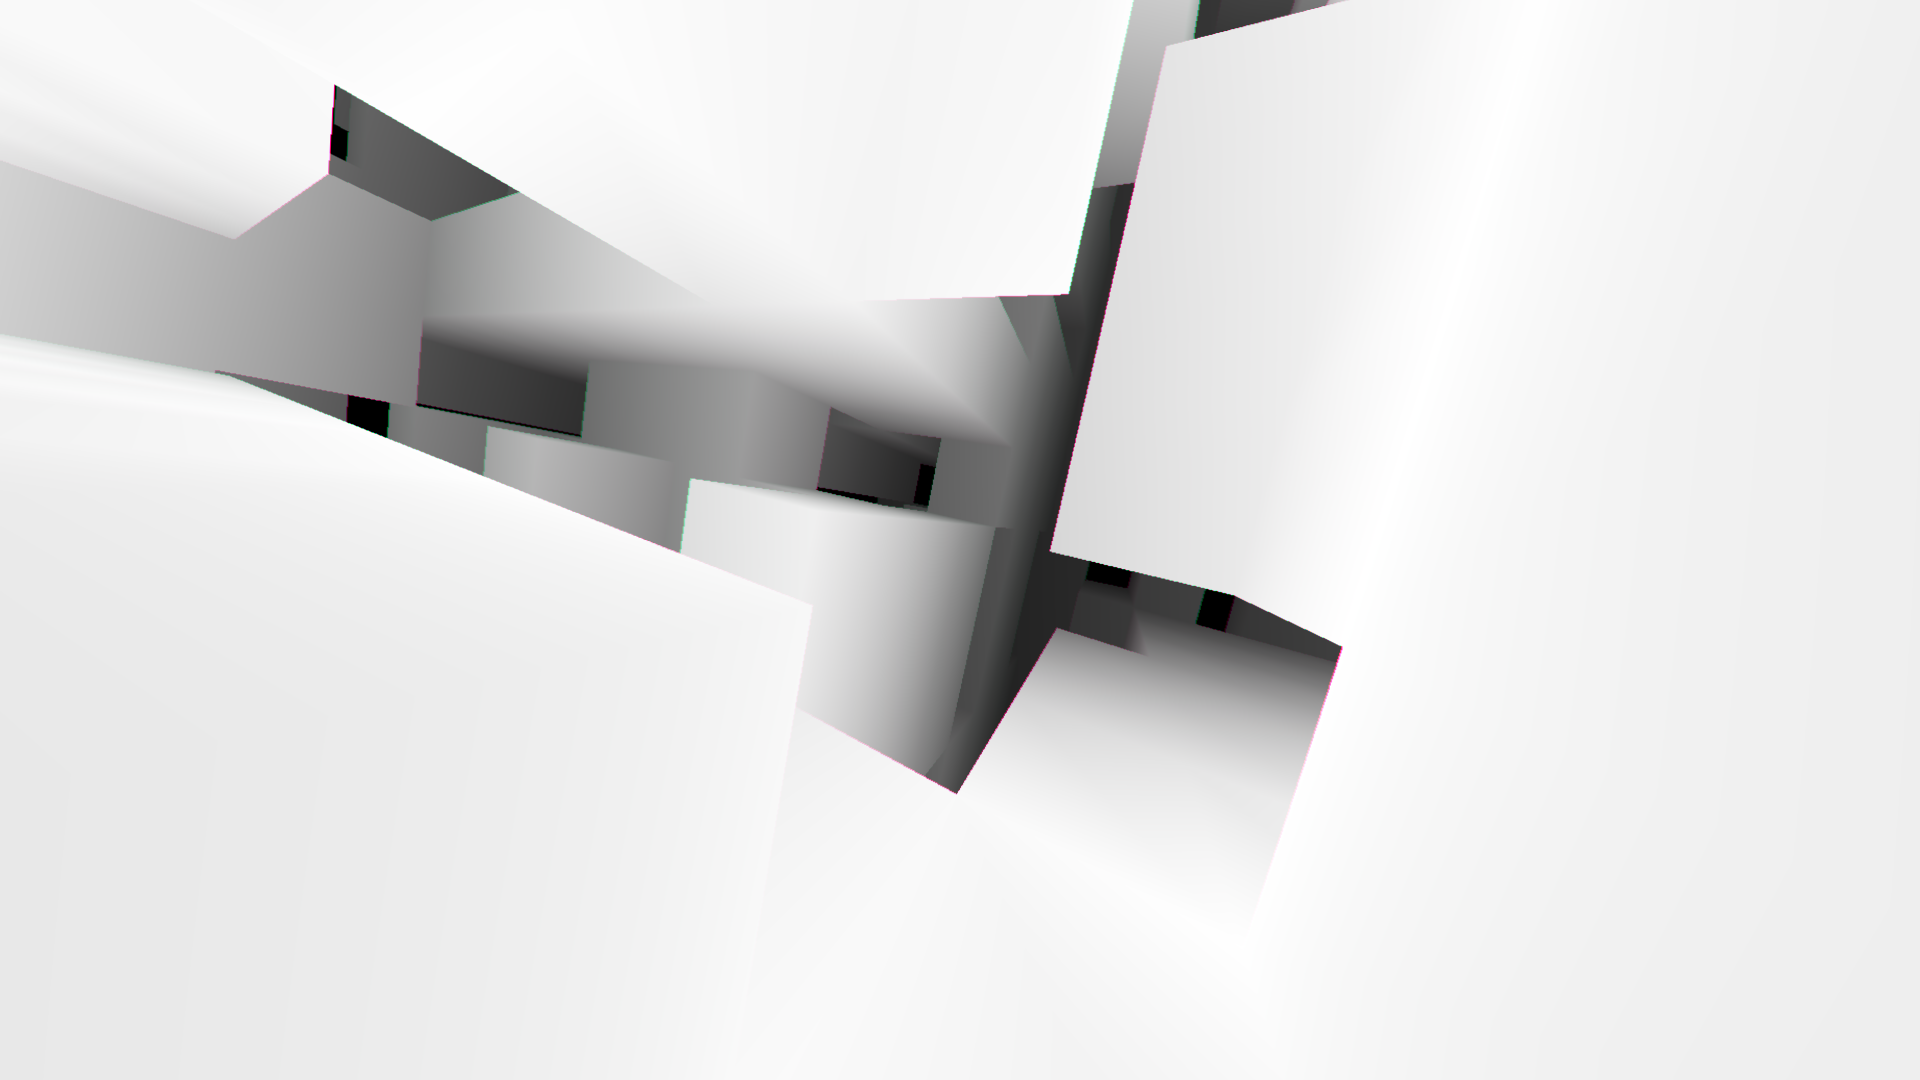
\includegraphics[width=0.49\textwidth]{axuy-grey.png}
  \includegraphics[width=0.49\textwidth]{axuy-turbo.png}
\end{center}

\section{Conclusion}

\begin{thebibliography}{69}
  \bibitem{cs5420} Sanjiv~K.~Bhatia.
    \href{http://www.cs.umsl.edu/~sanjiv/classes/cs5420/lectures/color.pdf}
         {``Color Image Processing''}.
    \emph{CS 5420: Digital Image Processing}.
    University Of Missouri---St.~Louis, Fall 2018.
  \bibitem{turbo} Anton Mikhailov.
    \href{https://ai.googleblog.com/2019/08/turbo-improved-rainbow-colormap-for.html}
         {\emph{Turbo, An Improved Rainbow Colormap for Visualization}}.
    Google AI Blog, August 20, 2019.
  \bibitem{rainbowbad} Noeska Smit.
    \href{https://medvis.org/2012/08/21/rainbow-colormaps-what-are-they-good-for-absolutely-nothing/}
         {\emph{Rainbow Colormaps---What are they good for? Absolutely nothing!}}
    medvis.org, August 21, 2012.
\end{thebibliography}
\end{document}
